\documentclass[a4paper,12pt]{article}

% Packages
\usepackage{graphicx}
\usepackage{amsmath}
%\usepackage[portuguese]{babel} % Set 'Portuguese' as document language
\usepackage{geometry}
\usepackage{fancyhdr}
\usepackage{setspace}
\usepackage{titlesec}  % For title formatting
\geometry{margin=1in}
\usepackage[labelfont = bf]{caption}
\usepackage[hidelinks]{hyperref}
\usepackage{float}
\usepackage{csquotes}
\usepackage{subcaption}
\bibliographystyle{unsrt}
\usepackage{hyperref}

\usepackage{soul}
\sethlcolor{black!5} % Defina a cor de destaque

\usepackage{listings}
\usepackage{xcolor}
\definecolor{structure}{HTML}{113b75}
\definecolor{blue}{HTML}{27607e} 

%\usepackage{inconsolata} % Pacote de fonte monoespaçada mais compacta
\lstset{
	basicstyle=\ttfamily\footnotesize,         % Fonte monoespaçada e menor
	numbers=none,                       % Sem números de linha
	backgroundcolor=\color{black!5},    % Cor de fundo clara
	frame=single,                       % Moldura ao redor do output
	breaklines=true,                    % Quebra de linha automática
	tabsize=2,                          % Tamanho da tabulação
	lineskip=-1pt,                      % Reduz o espaçamento entre linhas
	%columns=fullflexible,               % Reduz espaçamento entre caracteres
	showstringspaces=true              % mostrar espaços
	captionpos=b
}

%\setstretch{1}

\begin{document}

\begin{titlepage}
    \centering
    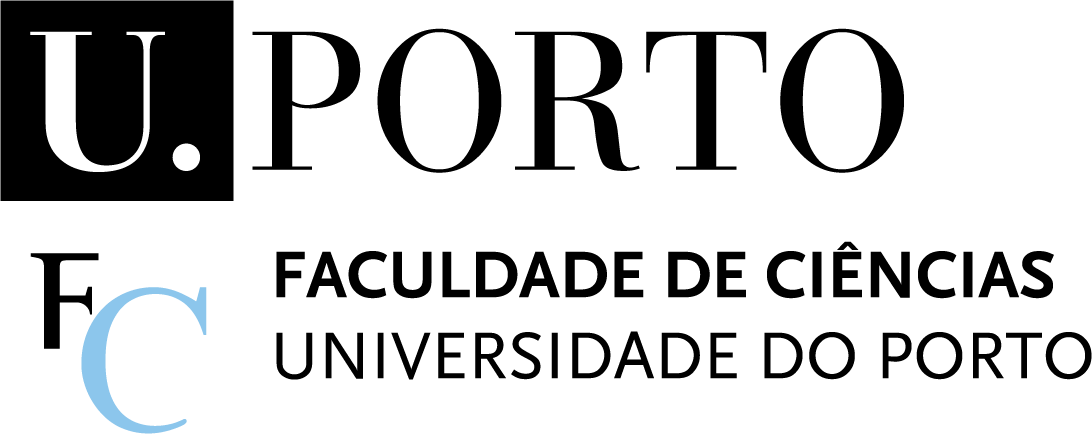
\includegraphics[width=6cm]{images/logo_fcup.png} 
    
\includegraphics[width=4cm]{images/logo_msi.png}
    \vspace{2cm}

\begin{center}
    {\Large \bfseries Segurança e Aplicações de Hardware Confiável}
    \vspace{1cm}
    \hrule 
    \vspace{0.5cm} 
    {\LARGE\bfseries Secure Data Lakes \par}
    \vspace{0.5cm}
    \hrule 
\end{center}

\vfill

    {\large \textbf{Maria Carreira up202408787 \\
    Matilde Simões up202108782 \\
    Ricardo Amorim up202107843} \par}
    \vspace{0.5cm}

    {\Large Março 2025 \par}
\end{titlepage}

\newpage

% Table of Contents
% Start page numbering from the Table of Contents
\setcounter{page}{1}  % Start counting from 1
\tableofcontents
\newpage


\section{Descrição do Problema}

%\cite{Nargesian2019}

%\begin{itemize}
%   \item Definição do que são Data Lakes.
%   \item Riscos e desafios associados ao armazenamento e processamento partilhado de dados.
%   \item Relevância do problema no contexto de dados médicos.
%   \item Exemplos de possíveis ataques ou falhas de segurança.
%\end{itemize}

\section[Visão Geral]{Visão Geral da Abordagem e do Hardware  \\ Confiável Adotado}

A utilização de \textit{hardware} confiável é essencial para garantir \textit{data lakes} seguros, especialmente quando se trata de dados sensíveis, como informações médicas. É fundamental garantir a segurança nestes ambientes, onde múltiplos utilizadores precisam do acesso aos dados agregados sem comprometer a privacidade individual. Uma das soluções mais eficazes para este tipo de problema é a utilização do \textit{Intel Software Guard Extensions (SGX)}, que é um ambiente de execução confiável (TEE) que permite o processamento seguro dos dados e protege contra diversos ataque, incluindo ataques provenientes de componentes com altos privilégios do sistema \cite{link}.

O \textit{Intel SGX} é uma tecnologia baseada em \textit{hardware} que possibilita a execução de código e o processamento de dados dentro de enclaves protegidos, o que impede acessos não autorizados e modificações indevidas.  A escolha do SGX justifica-se pelas seguintes vantagens:

\begin{itemize}
    \item Confidencialidade: Os dados dentro dos enclaves \textit{SGX} permanecem encriptados e inacessíveis, mesmo para administradores do sistema, prestadores de serviço \textit{cloud} ou atacantes com acesso privilegiado.
    \item Integridade: O ambiente de execução garante que apenas código confiável é executado dentro dos enclaves, prevenindo alterações não autorizadas.
    \item Verificação Remota: O \textit{SGX} fornece mecanismos para verificar a integridade e a autenticidade do código em execução dentro de um enclave. Este processo permite que um utilizador verifique a integridade do enclave antes de interagir com ele, assegurando que os dados processados não foram adulterados.
    \item Minimização da Superfície de Ataque: Ao isolar cálculos sensíveis do sistema operativo, o SGX reduz significativamente o risco de ataques, como a manipulação de memória, injeção de código e explorações ao nível do kernel.
\end{itemize}

Assim, o \textit{SGX} assegura que os enclaves são isolados e protegidos, permitindo que dados sensíveis sejam processados com segurança dentro do \textit{CPU}, sem ficarem expostos ao software privilegiado \cite{link}.

Os dados processados dentro dos enclaves \textit{SGX} estão protegidos contra acessos e modificações não autorizadas devido à estrutura da arquitetura que isola os enclaves em zonas protegidas da memória. Apenas o código autorizado dentro do enclave pode aceder e operar sobre os dados, impedindo que mesmo utilizadores com privilégios administrativos ou atacantes que comprometam o sistema operativo tenham acesso a informações confidenciais. Além disso, as chaves criptográficas utilizadas para proteger os dados nunca saem do enclave, eliminando riscos associados a ataques externos.

A confidencialidade dos dados é assegurada pelo \textit{Memory Encryption Engine (MEE)}, que protege as informações guardadas na \textit{Processor Reserved Memory (PRM)} contra acessos não autorizados \cite{link}. Os dados que se encontram fora do \textit{CPU} permanecem encriptados, garantindo que qualquer tentativa de leitura por parte do sistema operativo ou atacantes resulte apenas em informação ilegível. Apenas o \textit{CPU}, através do \textit{MEE}, é capaz de realizar a desencriptação em tempo real dos dados, garantindo que o único local onde podem ser lidos em texto claro é dentro do enclave, enquanto estão a ser processados.

A integridade dos enclaves é assegurada pelo mecanismo de verificação remota. Este mecanismo evita ataques como os \textit{rollback attacks}, que tentam reverter um enclave para um estado anterior e potencialmente comprometido que pode conter vulnerabilidades já corrigidas em versões mais recentes. Além disso, a criptografia aplicada pelo \textit{MEE} protege os dados contra ataques de extração de dados sensíveis diretamente da memória RAM, como os \textit{cold boot attacks}. Os dados guardados na \textit{DRAM} não desaparecem imediatamente após se desligar o sistema, logo um atacante pode tentar recuperá-los. Assim, o \textit{MEE} impede que informações sensíveis sejam recuperadas mesmo que um atacante tenha acesso físico ao hardware. 

Apesar da segurança avançada oferecida pelo \textit{SGX}, existem potenciais vulnerabilidades que podem ser exploradas para comprometer a sua proteção. Um dos principais desafios são os ataques de \textit{side channels} \cite{Brasser2017}, que podem extrair informações sensíveis ao analisar padrões de acesso à memória, medições de tempo de execução ou consumo de energia. Além disso, falhas no próprio código do enclave podem ser exploradas para executar instruções maliciosas e comprometer a segurança do sistema \cite{Schwarz2019}. Outras ameaças incluem enclaves maliciosos \cite{Aumasson2016}, que podem enganar aplicações legítimas e obter dados confidenciais, e ainda falhas na implementação do \textit{SGX}, como demonstrado em ataques como \textit{Foreshadow} \cite{foreshadow} \url{https://www.intel.com/content/www/us/en/security-center/advisory/intel-sa-00161.html}, que explora vulnerabilidades de microarquitetura para aceder a informações protegidas.

No contexto de \textit{data lakes} seguros, o \textit{SGX} possibilita a criação de uma base de dados remota mínima, onde múltiplos utilizadores podem armazenar e consultar informações com garantias de privacidade. Esta abordagem permite que consultas, como a análise de dados médicos, sejam processadas dentro dos enclaves, assegurando que apenas resultados agregados, como médias estatísticas, sejam expostos, sem revelar dados individuais. Além disso, facilita a partilha e colaboração segura entre diferentes entidades, como hospitais e instituições. Por fim, ao ser implementado em ambientes de \textit{cloud}, o \textit{SGX} protege as informações contra ameaças internas, garantindo que nem os próprios fornecedores de serviços conseguem aceder aos dados guardados.

Concluindo, a utilização do \textit{Intel SGX} neste projeto oferece garantias sólidas de segurança, confidencialidade e integridade. Através da aplicabilidade em ambientes de execução confiáveis, conseguimos implementar o  armazenamento e o processamento de dados sensíveis e ainda permitir a partilha de dados sem comprometer a privacidade. Esta abordagem garante que os dados permanecem sempre protegidos, mesmo em ambientes sujeitos a possíveis ameaças. Com os mecanismos de enclaves e verificação remota, o \textit{SGX} consegue garantir robustez para proteger \textit{data lakes}, especialmente em áreas críticas como a saúde.

\section{Abordagem Proposta}

\subsection{Visão Geral da Solução}
%\begin{itemize}
%   \item Proposta de utilização de enclaves SGX como elemento de confiança.
%   \item Justificação da escolha da tecnologia Intel SGX.
%\end{itemize}

\subsection{Entidades do Sistema}
%\begin{itemize}
%   \item Contribuintes de dados (e.g., hospitais).
%   \item Sistema de gestão da base de dados.
%   \item Clientes/consultores (entidades que realizam queries).
%   \item Enclaves SGX como núcleo seguro do sistema.
%\end{itemize}

\subsection{Arquitetura Geral}
%\begin{itemize}
%    \item Diagrama (recomendado).
%    \item Explicação do fluxo: Ingestão de dados → Processamento seguro → Resultados %agregados.
%\end{itemize}

\section{Requisitos Funcionais e de Segurança do Projeto}

\section{Descrição do progresso feito e Próximos objetivos}

% Bibliography
\bibliography{references}

\end{document}
